%%%%%%%% ICML 2026 SENPAI SUBMISSION %%%%%%%%%%%%%%%%%

\documentclass{article}

\usepackage{microtype}
\usepackage{graphicx}
\usepackage{subcaption}
\usepackage{booktabs}
\usepackage{multirow}
\usepackage{array}
\usepackage{enumitem}
\usepackage{float}
\usepackage{amsmath}
\usepackage{amssymb}
\usepackage{mathtools}
\usepackage{amsthm}
\usepackage{xurl}
\usepackage{hyperref}
\usepackage[capitalize,noabbrev]{cleveref}

\newcommand{\theHalgorithm}{\arabic{algorithm}}
\newcommand{\best}[1]{\textbf{#1}}

% Use preprint mode so author names render in the local preview PDF.
\usepackage{icml2026/algorithm}
\usepackage{icml2026/algorithmic}
\usepackage[preprint]{icml2026/icml2026}
\usepackage{newtxtext}

\usepackage[disable,textsize=tiny]{todonotes}

\icmltitlerunning{\scriptsize SENPAI}

\begin{document}

\twocolumn[
  \icmltitle{SENPAI: Self-ExperimentatioN for Physical AI\\
  An Observability-Based Research Harness}

  \icmlsetsymbol{equal}{*}

  \begin{icmlauthorlist}
    \icmlauthor{Thomas Capelle}{equal,wandb}
    \icmlauthor{Morgan McGuire}{equal,wandb}
    \icmlauthor{Justin Hodges}{coreweave}
  \end{icmlauthorlist}

  \icmlaffiliation{wandb}{Weights \& Biases, San Francisco, CA, USA}
  \icmlaffiliation{coreweave}{CoreWeave, Roseland, NJ, USA}
  \icmlcorrespondingauthor{Morgan McGuire}{morg@wandb.com}
  \icmlkeywords{Autonomous research, CFD surrogates, ML systems, agent observability, AI for science}

  \vskip 0.3in
]

\printAffiliationsAndNotice{\icmlEqualContribution}

\begin{abstract}
SENPAI (Self-Experimentation for Physical AI) is an observability-first research harness in which multi-agent state is grounded in pull requests and structured experiment logs rather than agent memory and scratchpads. Although task-agnostic, we evaluate SENPAI on CFD-surrogate recipe search, where performance depends on architecture, optimization, losses, normalization, and physics-aware considerations. SENPAI uses a thin Advisor/Student loop to turn hypotheses into PRs, training runs, and PR comments, producing an experiment ledger queryable by both agents and researchers. This makes experiments auditable, recoverable, and human-steerable. We evaluate Transolver-based SENPAI across DrivAerML, AirfRANS, and TandemFoilSet. Starting from the original Transolver model, SENPAI improves DrivAerML surface-pressure and wall-shear-stress relative-$L_2$ error, reduces AirfRANS surface-MSE below all compared references, and reaches lower TandemFoilSet cruise-random-uniform normalized full-field MSE than the reported benchmark. Overall, SENPAI supports sparsely steered, multi-day semi-autonomous research that can deliver strong task-specific models. We release the harness and public GitHub/W\&B experiment ledger.
\end{abstract}

\section{Introduction}

CFD surrogates offer a way to accelerate engineering design: learned models can screen early-stage geometries, explore operating regimes, and focus expensive CFD or physical testing on the most promising candidates. Recent surrogate models now handle larger meshes, irregular geometries, stricter accuracy targets, and smaller training sets than were feasible only a few years ago \citep{zhou2026transolver3}, making hybrid ML-CFD workflows increasingly attractive.

In practice, however, training a useful CFD surrogate is still a niche capability. Performance depends on architecture, optimization, normalization, boundary conditions, symmetries, and rollout stability \citep{wang2024cfdmlsurvey}. Strong recipes require both ML expertise and domain knowledge in aerodynamics or fluid dynamics \citep{hodges2024cfdmlmonograph}, which many engineering teams do not have. SENPAI targets this gap by exploring, documenting, and refining problem-specific surrogate recipes while keeping researchers in the loop.

Recent autonomous-research systems show that LLM agents can search literature, propose hypotheses, edit code, run experiments, and produce reports \citep{lu2024aiscientist,schmidgall2025agentlaboratory,yamada2025aiscientistv2,miyai2026jraiscientist}. SENPAI builds on this direction but focuses on a different systems question: how should long-running, multi-experiment ML research be represented so that both agents and researchers can audit, recover, compare, and steer it?

SENPAI's central design choice is to leverage the systems of record ML teams already use as the foundation of a research agent: git commits and pull requests for hypothesis development, code review, and discussion \citep{githubdocs_pullrequests}; git history for ordered provenance \citep{chacon2014progit}; and an experiment tracking tool for training configurations, metrics, model checkpoints, and system traces \citep{biewald2020wandb,wandbdocs_experiments}. Each hypothesis, code diff, training result, review decision, failed run, and baseline update becomes both machine-queryable and research-reviewable through these existing tools.

The harness loop is deliberately thin. An Advisor reads the current experiment ledger, proposes a literature-grounded hypothesis as a draft PR, and assigns it to a GPU-backed Student. The Student checks out the branch, modifies the training code, runs the experiment, logs metrics to W\&B, and reports results in the PR. The Advisor then merges, requests revision, or closes the line of inquiry. Humans can steer the Advisor or Student through GitHub issues and PR comments, while markdown scratchpads remain secondary sources of state rather than the primary system of record.

Across the research programme, SENPAI produced more than 2,700 agent-generated PRs, 11,000 W\&B runs, and operated with up to 59 concurrent Student agents, turning a multi-week semi-autonomous research programme into a durable experiment ledger.

\paragraph{Contributions.}
\textbf{Observability-first research harness.} We introduce and open-source SENPAI, a semi-autonomous ML research harness that grounds experiment state in PRs, commits, and W\&B runs, producing a ledger that is queryable by agents and inspectable by researchers.

\textbf{CFD-surrogate recipe search.} Starting from Transolver-style baselines, SENPAI discovers improved recipes across AirfRANS, DrivAerML, and TandemFoilSet, with strongest gains on surface quantities.

\textbf{Failure-mode analysis.} We analyze a 24-hour fleet trace with 53,022 Claude requests and 5.24B tokens, showing that the dominant failures were monitor-driven context bloat, brittle tool interfaces, checkpoint/result-capture gaps, and state reconciliation issues rather than failures of scientific reasoning.

\section{Related Work}

Recent autonomous-research systems show that LLM agents can search literature, propose hypotheses, edit code, run experiments, and produce research reports. The AI Scientist generates ideas, implements experiments, writes papers, and runs automated review \citep{lu2024aiscientist,sakana2024aiscientist}, while AI Scientist-v2 extends this direction with agentic tree search and workshop-level paper generation \citep{yamada2025aiscientistv2,sakana2025aiscientistv2}. Agent Laboratory structures literature review, experimentation, and report writing around a researcher-provided idea \citep{schmidgall2025agentlaboratory}, and Jr. AI Scientist iteratively improves a baseline paper using modern coding agents \citep{miyai2026jraiscientist}. Related systems emphasize collaboration, shared artifacts, or domain tools: ResearchAgent generates and revises ideas over scientific-literature graphs \citep{baek2024researchagent}, AgentRxiv lets agent laboratories upload and retrieve generated reports from a shared preprint server \citep{schmidgall2025agentrxiv}, ChemCrow and Coscientist connect LLM planners to chemistry tools and laboratory workflows \citep{bran2024chemcrow,boiko2023coscientist}, and FunSearch couples an LLM generator to a verifiable evaluator and scored program database \citep{romeraparedes2024funsearch}. Similarly, in general ML engineering, Hugging Face's \texttt{ml-intern} is a recent, non-science-focused example that reviews papers, writes training code, and runs experiments \citep{huggingface2026mlintern}. These systems establish the value of tool use, execution, and persistent artifacts in autonomous research. SENPAI builds on that direction, but studies a different substrate question: how should the state of a long-running, multi-experiment ML research programme be represented so that both agents and researchers can inspect, compare, recover, and steer it?

The closest systems to SENPAI also recognize that long-horizon agents need state outside the model context, but they choose different substrates. Kosmos maintains an internal structured memory of literature-search and data-analysis summaries to choose later tasks, and cites final report claims with papers or generated Jupyter notebooks \citep{mitchener2025kosmos}. AiScientist uses a permission-scoped File-as-Bus workspace so agents can re-ground on file-based analyses, plans, code, logs, and experimental evidence \citep{chen2026aiscientist}. Grounded autonomous research externalizes state as rerunnable simulation artifacts and comparison results within a single-paper reproduction loop \citep{huang2026groundedautonomousresearch}. SENPAI takes a complementary systems position: the authoritative state should be the MLOps tooling machine learning researchers already use. In SENPAI, pull requests carry hypotheses, code review, discussion, and review decisions \citep{githubdocs_pullrequests}; git history provides ordered code provenance \citep{chacon2014progit}; and experiment trackers such as Weights \& Biases store metrics, hyperparameters, system metrics, checkpoints, and agent traces \citep{biewald2020wandb,wandbdocs_experiments}. This distinction matters most at scale: once an autonomous research system produces hundreds or thousands of experiments, the central challenge is no longer only whether an agent can run an effective experiment, but whether researchers can understand the programme it is creating.

\section{Methodology: System Design}

SENPAI's central design principle is that authoritative experiment state lives in pull requests, git history, and W\&B runs, not in agent memory or local scratchpads. The harness is therefore organized around making each hypothesis, code change, training result, and review decision durable, queryable, and inspectable through existing research tools.

\begin{figure}[t]
  \centering
  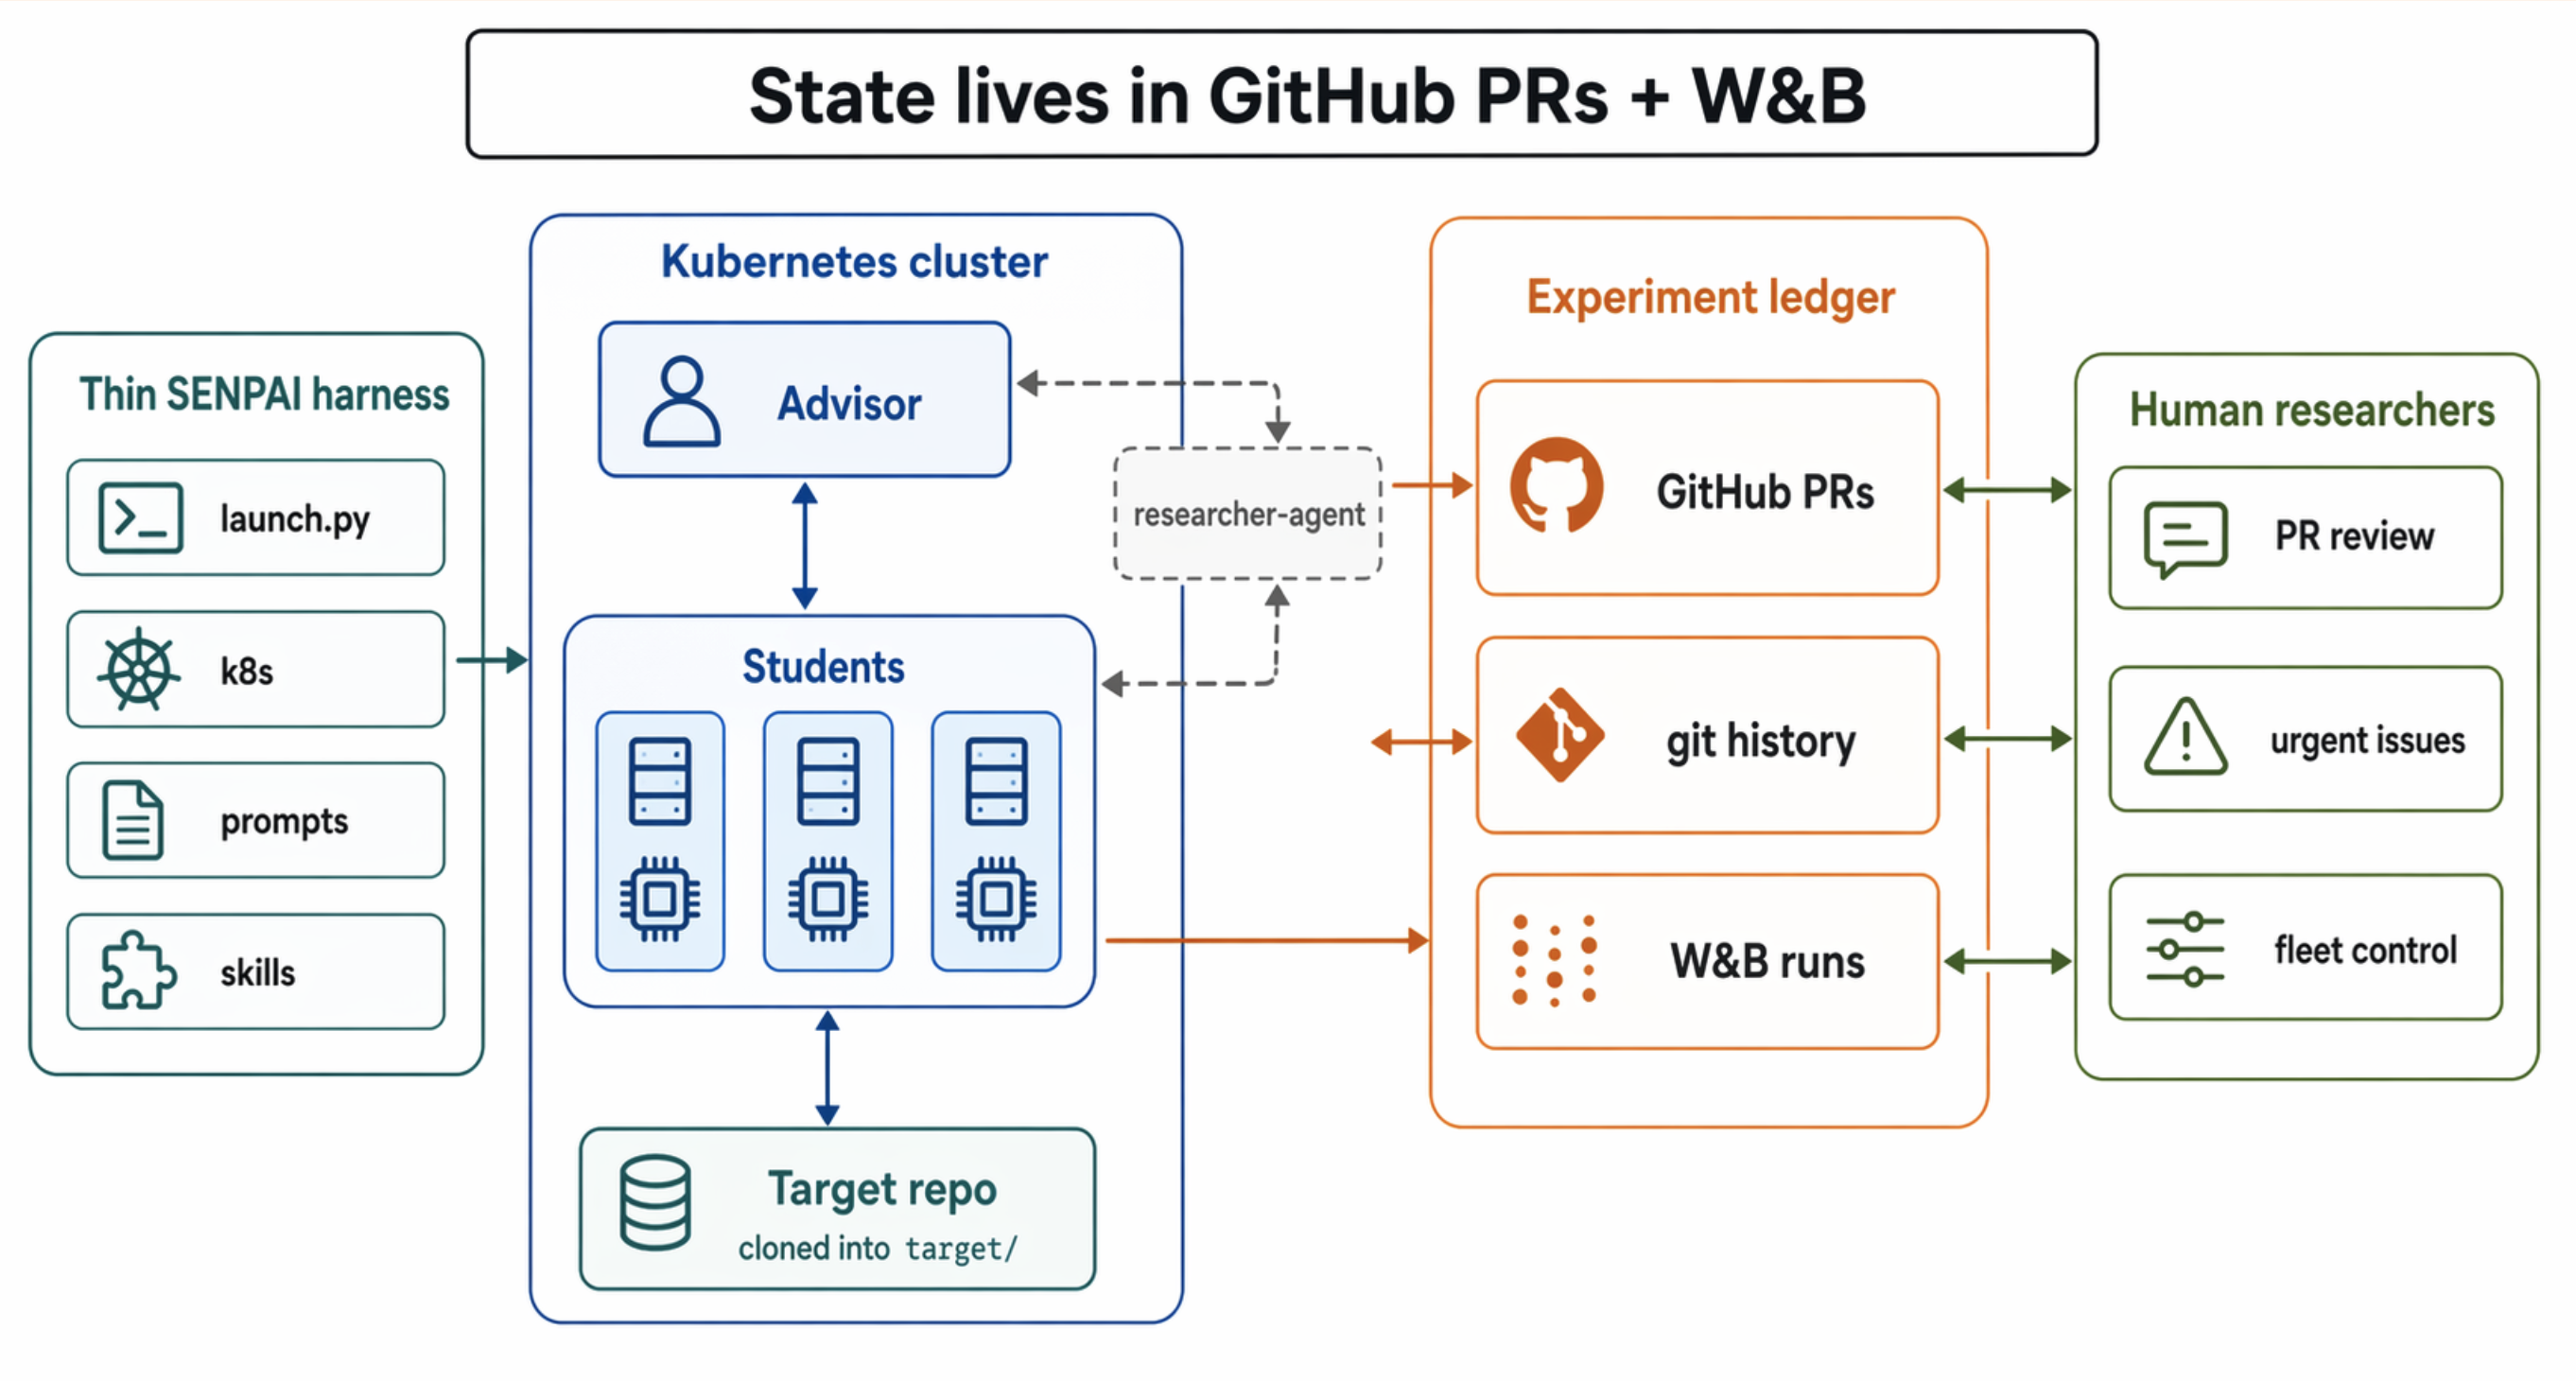
\includegraphics[width=\columnwidth]{section2_image.png}
  \caption{SENPAI deployment architecture. A thin harness deploys one Advisor and $N$ Student pods; both roles can call a shared literature-search sub-agent. All programme state lives outside the cluster in the experiment ledger: GitHub PRs, git history, and W\&B runs.}
  \label{fig:architecture}
\end{figure}

SENPAI is a thin two-role harness over a task repository. An Advisor reads the current experiment ledger, optionally calls a literature-search sub-agent, opens draft PRs containing hypotheses and experiment instructions, and assigns them to GPU-backed Students. Each Student claims its labeled PR, edits the branch, launches training with W\&B logging, and reports results back as PR comments. Researchers can steer Advisors or Students via labeled GitHub issues or by leaving comments on a PR. A hypothesis's trajectory therefore remains visible as a standard PR history linked to experiment-tracker runs, rather than as an agent-internal trace.

SENPAI follows three design choices: externalizing experiment state into existing systems of record, keeping the autonomous loop thin, and exposing the same ledger to both agents and researchers.

\subsection{Externalized Experiment State}

The experiment ledger has two linked records. The PR records the qualitative trajectory: hypothesis, implementation instructions, code diff, Student report, Advisor review, and final decision. W\&B records the quantitative trajectory: configuration, metrics, checkpoints, system data, and agent traces. Together these records are inspectable through familiar GitHub and W\&B interfaces and queryable through mature CLIs, allowing both researchers and agents to audit individual experiments or summarize programme-level progress.

The Advisor also maintains lightweight markdown summaries for focus, such as current baseline metrics, dataset notes, and open research directions. These files are treated as caches rather than authoritative state: when summaries disagree with PRs, git history, or W\&B runs, the ledger wins.

\subsection{Thin Advisor/Student Loop}

Each experiment follows a PR-mediated lifecycle. The Advisor drafts a PR with a hypothesis, implementation guidance, target metrics, baseline values, and a Student label. The Student implements the change on the PR branch, runs training with W\&B logging, and posts commands, training run links, metrics, and experiment interpretation as a PR comment. Once the PR is marked ready for review, the Advisor compares the result against the stated baseline and either merges the improvement, requests revision, or closes the branch. Merged PRs advance the programme baseline used for subsequent hypotheses.

SENPAI deploys as a small set of Kubernetes workloads: one Advisor CPU pod, $N$ Student GPU pods, and a shared persistent data volume for datasets and checkpoints. The harness image is stable across problems; a task repository can be swapped in per SENPAI research programme, so every agent commit, branch, and PR lives in a self-contained target repository that a researcher can inspect independent of the harness.

The outer harness loop is programmatic rather than agentic. A shell wrapper polls GitHub and Student state for review-ready PRs, human issues, new comments, and idle Students; if no action is available, it sleeps without invoking the LLM. When action is required, the wrapper starts or resumes the Advisor with a triage message. This keeps routine polling outside the model context and focuses the agent on research decisions rather than heartbeat bookkeeping.

\subsection{Shared Observability}

Researchers primarily steer SENPAI's Advisor or Students through GitHub issues, while PR comments can also provide experiment-level intervention. This channel is intentionally low bandwidth: SENPAI is designed for sparse steering rather than continuous supervision, and each intervention remains attached to the public experiment record it affected.

\section{Experiments and Results}

\begin{figure*}[t]
  \centering
  
\includegraphics[width=0.98\textwidth]{icml2026/figures/drivaerml_surface_pareto/drivaerml_surface_pressure_pareto.pdf}
  \caption{Evolution of DrivAerML surface-pressure test error across two SENPAI campaigns. Faded markers show individual completed experiments from the \texttt{yi} and \texttt{tay} branches, while solid curves show the cumulative Pareto frontier: the best surface-pressure relative $L_2$ error achieved up to each experiment count. The vertical lines mark GitHub-recorded human researcher/operator interventions. \texttt{tay} was instructed to use DDP8 and was given a 6 hour per-experiment training budget, hence the better performance.}
  \label{fig:drivaerml-surface-pareto}
\end{figure*}

\subsection{Experiment Setup}

Claude Code (v2.1.85 to v2.1.117) was run in headless mode as the agent harness for both the Advisor and Students. Claude Opus 4.6 and Claude Opus 4.7 were used with a compaction trigger at 200k tokens. Student pods were scheduled on NVIDIA RTX 6000 Blackwell nodes with 96 GB VRAM per GPU, from 1 to 8 GPUs per Student node. At maximum, $N=59$ concurrent Students were tested, with peak concurrent training runs of 347. Over the five-week experimentation and harness-development cycle, 29 billion tokens were processed by Claude Code while running physical-AI experiments.

Over the course of the research programme, SENPAI created more than 3,000 experiment PRs and recorded over 11,000 W\&B runs while deploying, at peak, 59 distinct Student agents. Approximately 30B Claude Code tokens were processed during experimentation.

\subsection{Data and Benchmarks}

To demonstrate SENPAI's CFD performance across multiple benchmarks, we train and evaluate on three CFD surrogate datasets spanning 2D tandem-airfoil flow, 2D airfoil RANS, and 3D automotive aerodynamics: TandemFoilSet \citep{lim2026tandemfoilset}, AirfRANS \citep{bonnet2022airfrans}, and DrivAerML \citep{ashton2024drivaerml}.

\paragraph{TandemFoilSet.}
We use the paper's original Experiment 4 partition, Cruise Random and Race Car tasks, as one of two TandemFoilSet datasets and measure denormalized surface-pressure MAE. In addition, we introduce a second dataset split, TandemFoilSet-Balanced \citep{mcguire2026tandemfoilsetbalanced}, with 1,499 training cases across four balanced test splits: one single-foil in-distribution split, two unseen-front-camber geometry holdouts (race-car and cruise), and one Reynolds-number holdout. An equal-weight average denormalized surface-pressure MAE of these four splits is used as the test metric.

\paragraph{AirfRANS.}
We use the official full task with the last 10\% of the official training list held out for validation, giving a 720/80/200 train/validation/test split while keeping the official test set unchanged. We test on normalized targets on the official test split.

\paragraph{DrivAerML.}
We use the public surface split on the available processed cases, 400/34/50 train/validation/test, and measure surface-pressure relative-$L_2$ in percent, computed per case on unnormalized predictions and targets and then averaged over test cases.

\subsection{DrivAerML: Preliminary Surface-Pressure Transfer Result}

On the DrivAerML benchmark, SENPAI, starting from a Transolver-based implementation, improves on the original Transolver's test-set metrics of surface-pressure relative-$L_2$ error (3.98\% versus 4.81\%) and vector wall-shear-stress relative-$L_2$ error (7.31\% versus 8.95\%). \Cref{fig:drivaerml-surface-pareto} shows the autonomous experiment trajectory for surface-pressure test error across the main DrivAerML branches.

\begin{table}[H]
  \caption{DrivAerML test relative-$L_2$ error (\%). Lower is better; bold marks the best value in each metric column.}
  \label{tab:drivaerml}
  \centering
  \small
  \setlength{\tabcolsep}{3pt}
  \begin{tabular}{@{}lrrr@{}}
    \toprule
    Method & $p_s$ & $\tau$ & $p_v$ \\
    \midrule
    SENPAI, ensemble & \best{3.69} & 6.86 & 11.36 \\
    Transolver-3 \citep{zhou2026transolver3} & 3.71 & \best{5.85} & \best{5.72} \\
    AB-UPT \citep{alkin2025abupt} & 3.82 & 7.29 & 6.08 \\
    SENPAI, single model & 3.98 & 7.31 & 11.33 \\
    Transolver++ & 4.12 & 6.42 & 6.70 \\
    Transolver \citep{wu2024transolver} & 4.81 & 8.95 & 7.74 \\
    \bottomrule
  \end{tabular}
\end{table}

The final training recipe SENPAI found used the original Transolver backbone but scaled it to 4 layers, 512 hidden units, and 128 slices, replaced fixed sinusoidal coordinates with a separable learnable Fourier positional embedding initialized across multiple spatial scales \citep{li2021learnable,schenck2025learningropes}, and trained with Lion \citep{chen2023symbolic} plus EMA. It also added physics-preserving $y$-plane reflection augmentation, flipping the lateral coordinate, surface-normal $n_y$, volume-coordinate $y$, and wall-shear $\tau_y$ sign, and trained for 50 epochs with 8-GPU DDP for an effective batch size of 16. A notable empirical finding from SENPAI was the application of this lightweight STRING-inspired encoding from computer vision and robotics use cases to CFD surrogate modelling.

Finally, a separate 50-epoch ensemble trained by SENPAI improved on all reported surface-pressure relative-$L_2$ metrics for DrivAerML (3.69\%) and improved on AB-UPT for wall-shear relative-$L_2$ error (6.86\%). A large gap in test-set volume-pressure relative-$L_2$ error was observed relative to AB-UPT and Transolver-3, potentially in part due to the shorter training time of SENPAI compared to the 500-epoch trainings of AB-UPT and Transolver-3. This training-duration discrepancy highlights an important decision criterion in autonomous research training: whether to scale up to longer, more expensive training runs after observing promising smaller-scale experimental results.

\subsection{AirfRANS}

On the AirfRANS full benchmark, SENPAI, starting from a Transolver-based implementation, improves substantially on the original Transolver surface-MSE result (5-seed mean 0.0013 versus 0.0142) and on the strongest published surface reference, SpiderSolver (0.0043). The same model obtains mean volume-MSE of 0.00451, improving on GeoANF but remaining above SpiderSolver and slightly above the original Transolver volume result. SENPAI therefore achieves the strongest reported surface-MSE among these references, while the full benchmark remains limited by volume accuracy.

\begin{table}[H]
  \caption{AirfRANS full-task test MSE. Targets are train-statistic normalized, per-case means on the official test split; lower is better; bold marks the best value in each metric row. Spider denotes SpiderSolver \citep{qi2025spidersolver}.}
  \label{tab:airfrans}
  \centering
  \small
  \setlength{\tabcolsep}{2.5pt}
  \begin{tabular}{@{}lrrrr@{}}
    \toprule
    Metric & SENPAI & Spider & GeoANF & Transolver \\
    \midrule
    Surface MSE & \best{0.00130} & 0.0043 & 0.0089 & 0.0142 \\
    Volume MSE & 0.00451 & \best{0.0017} & 0.0062 & 0.0037 \\
    \bottomrule
  \end{tabular}
\end{table}

The final AirfRANS recipe SENPAI found used a 2-layer, 256-hidden-unit, 4-head SENPAI-Transolver with 96 slices, fixed multiscale Fourier coordinate features, a zero-initialized surface refinement head, Lookahead-wrapped AdamW, cosine scheduling, gradient clipping, weight decay, EMA with target decay 0.999, and a volume-weighted normalized-MSE objective with volume loss weight 10.0. All five seeds beat the published SpiderSolver surface-MSE result, while volume-MSE remains above SpiderSolver and more sensitive to seed.

\subsection{TandemFoilSet}

Under the TandemFoilSet Experiment-4 task, SENPAI found a Transolver-based improvement on the cruise random uniform full-field MSE of the original paper ($1.7\cdot 10^{-3}$ versus $1.0\cdot 10^{-1}$). On TandemFoilSet-Balanced, SENPAI found a recipe that produced a denormalized surface-pressure MAE of 23.45 using a 5-seed average.

\begin{table}[H]
  \caption{TandemFoilSet-Balanced 5-seed mean denormalized surface-pressure MAE. Lower is better.}
  \label{tab:tandem-balanced}
  \centering
  \small
  \begin{tabular}{@{}lr@{}}
    \toprule
    Metric & MAE \\
    \midrule
    Single-foil in-distribution & 17.2905 \\
    Race-car camber holdout & 31.2177 \\
    Cruise camber holdout & 28.3145 \\
    Reynolds-number holdout & 16.9834 \\
    Average & 23.4515 \\
    \bottomrule
  \end{tabular}
\end{table}

The PR ledger shows the path: lower learning rates near \texttt{1e-4}, gradient clipping, EMA, warmup, and schedule-length tuning. A separate no-W\&B TandemFoilSet-Balanced audit reached \texttt{test\_avg/mae\_surf\_p = 27.2125} in PR \#1285, beating the \texttt{40.927} target by \texttt{13.7145}, supporting the same schedule-and-throughput conclusion under a separate audit lane.

\subsection{Ablating Centralized Experiment Logging}

To investigate the role of centralized experiment observability, an ablation compared SENPAI with hosted experiment logging against SENPAI using only locally written experiment results. Both settings used a 12-hour outer-loop budget and a 30-minute per-experiment cutoff. SENPAI's local-only logging trial achieved the strongest average final performance on TandemFoilSet-Balanced across five 12-hour trials, but with substantially higher variance, including one trial that failed to log a valid test-set result.

For the hosted-W\&B Willow arm, \cref{fig:willow-sankey} summarizes how PR-indexed hypotheses moved from Advisor branches through experiment families to final PR outcomes.

\begin{figure*}[t]
  \centering
  
\includegraphics[width=0.92\textwidth]{icml2026/figures/willow_sankey/willow_simplified_sankey.pdf}
  \caption{Experiment-ledger flow for the hosted-W\&B Willow ablation arm on TandemFoilSet-Balanced. Five Advisor branches (A1--A5) are routed through PR-indexed hypothesis families and into final PR outcomes; ribbon width is proportional to PR count. The figure compresses 167 GitHub-mediated experiments into a researcher-readable audit map, showing where autonomous search effort was allocated and how it resolved into merged, closed, or still-open work.}
  \label{fig:willow-sankey}
\end{figure*}

\begin{table}[H]
  \caption{Experiment-logging ablation on TandemFoilSet-Balanced. Surface-pressure MAE; lower is better. Bold marks the better value for Best test and Mean test.}
  \label{tab:logging-ablation}
  \centering
  \small
  \begin{tabular}{@{}lrr@{}}
    \toprule
    Metric & Hosted log. & Local-only \\
    \midrule
    Best test & 44.15 & \best{27.21} \\
    Mean test & 51.23 & \best{45.10} \\
    SD & 4.79 & 12.89 \\
    \bottomrule
  \end{tabular}
\end{table}

Analyzing the Claude Code logs, agents with hosted logging more often verified run histories, compared split-level metrics, checked seed/control behavior, and reasoned about stale branches before accepting results. This produced a cleaner audit trail and more consistent provenance. The local-only arm was less verification-oriented, referencing keywords related to seeds and experimental variance roughly $3\times$ less. While the local-only arm achieved a strong average result, over longer experiment durations the performance of this setup is likely to drift.

\begin{table}[H]
  \caption{Behavioral differences in the experiment-logging ablation.}
  \label{tab:logging-behavior}
  \centering
  \small
  \begin{tabular}{@{}p{0.48\columnwidth}rr@{}}
    \toprule
    Behavior & With log. & No log. \\
    \midrule
    Tool calls & 60,600 & 78,372 \\
    Tool errors / 1k calls & 63.10 & 32.23 \\
    Seed/variance refs. / 1k records & 55.04 & 17.61 \\
    PRs opened & 187 & 167 \\
    PR merge rate & 31.0\% & 23.5\% \\
    Median result-to-merge latency & 0.294 h & 0.162 h \\
    \bottomrule
  \end{tabular}
\end{table}

\subsection{Flat-Agent Comparison}

To contrast SENPAI's Advisor-mediated loop, we compared the performance of a \texttt{kagent} harness \citep{kagent2026} against the SENPAI harness using the TandemFoilSet-Balanced dataset and the same compute budget. \texttt{kagent} is a lighter-weight harness that drops the Advisor/Student split in favor of a flat Kaggle-like competition with a shared leaderboard; each agent keeps its own experiment journal and is prompted to compete aggressively to climb the leaderboard. In contrast to a Kaggle competition, the agents also have access to the same W\&B project and commit history, so they can learn from other agents' work.

\begin{table}[H]
  \caption{TandemFoilSet-Balanced 12-hour harness comparison. Lower average surface-pressure MAE is better; bold marks the best value in the metric row.}
  \label{tab:kagent}
  \centering
  \small
  \begin{tabular}{@{}lrr@{}}
    \toprule
    Metric & SENPAI & \texttt{kagent} \\
    \midrule
    Best avg-surf-$p$ MAE & 44.15 & \best{34.58} \\
    \bottomrule
  \end{tabular}
\end{table}

In a direct 12-hour head-to-head, \texttt{kagent} behaved like a public Kaggle sprint: agents trained short variants, watched the leaderboard and shared W\&B configs, and quickly reused recipes that worked for peers. This fast peer diffusion, including copied hyperparameters and occasional prediction ensembles, likely gave it an exploitation-speed edge over SENPAI's slower PR-mediated review loop. While this was successful in a 12-hour experiment setting, the inability to steer these agents and the less rigorous polling and monitoring infrastructure are likely to lead to drift and context rot as each Claude Code agent's context window fills.

\section{Discussion}

\subsection{Observable State as a Control Surface}

The PR and W\&B ledger made SENPAI useful as a research assistant rather than a tool to execute experiments. Because hypotheses, code diffs, metrics, failures, and review decisions were all recorded in systems researchers already use, humans could inspect the research programme without needing to read the agents' context. The same records also gave agents a stable system of record: they could query prior runs, identify stale experiments, compare seed behavior, and decide whether a new result actually advanced the baseline. In SENPAI, observability is therefore not simply logging; it is the layer through which both humans and agents can steer the research programme.

This externalized state also reduced the fragility of long-running agent sessions. When agents compacted, restarted, or lost local scratchpad context, the next cycle could reconstruct the experiment from the PR description, code diff, git history, W\&B runs, and posted result comments. Local summaries remained useful for focus, but they were treated as caches over a more durable experiment record.

The ledger also turned a collection of individual experiments into a queryable research programme. Researchers and agents could ask what had been tried, which failures were informative, which recipes transferred across datasets, where progress had stalled, and which resources were idle. This is SENPAI's central systems claim: the goal is not to replace the researcher, but to increase the bandwidth at which researchers can understand, guide, and accelerate experimentation.

\subsection{Harness Tradeoffs}

The \texttt{kagent} comparison highlights a harness-design tradeoff. Flat, leaderboard-driven cohorts can share successful recipes quickly because agents observe peer results directly and optimize for short-horizon score improvement. In contrast, SENPAI's PR-mediated loop is slower but preserves review decisions, experiment provenance, and sparse human steering. We view \texttt{kagent} as useful for rapid exploitation, and SENPAI as better suited to longer-running programmes where auditability and recovery matter alongside score.

\subsection{Failure Modes: Where Long-Running Research Agents Break}

SENPAI's most common failures were harness-engineering failures: monitoring long-running jobs, recovering across compaction or restarts, enforcing brittle tool interfaces, and reconciling PR state with W\&B state. They were less often failures of scientific reasoning. This distinction matters because it suggests that improving autonomous research systems requires better observable infrastructure, not only stronger prompts or more capable models.

During development, one dominant cost to running SENPAI was monitor-driven context bloat. In one notable experiment, Students monitored training logs for progress, errors, checkpoints, and completion, but persistent \texttt{tail -f | grep} events repeatedly resumed long-lived Student sessions for low-information log lines. In a 24-hour window with 57 Students running, 615 monitor setups produced 28,247 agent-facing monitor events and 28,246 agent responses, consuming 3.25B cache-inclusive tokens. The median agent response reloaded roughly 110k cached tokens while adding only 347 new uncached input tokens. This is an example of an architectural failure mode when running long-running research systems: training monitors should be cheap and escalation-based, surfacing only relevant events such as errors, experiment completion, or metric milestones.

Tool-use errors were smaller but systematic: in the same 24-hour window, 892 of 25,365 tool results had errors. The main causes were failed shell commands, GitHub scope errors, blocked wait patterns, wrong paths, failed pushes, oversized reads, and edit-guard failures. These errors point to a practical lesson: high-frequency harness operations should be executable helpers with narrow interfaces, rather than repeatedly reconstructed shell or GitHub operations inside agent context.

Compaction introduced a separate risk. The 24-hour window contained 240 automatic compactions across the 57 Students, with Student contexts reduced from roughly 196k tokens to 3k-token summaries. These summaries were sufficient for resumption, but lossy: state drift appeared in the agent conversation logs with mistakes such as incorrect GitHub labels or confusion over live experiment state. SENPAI's experiment ledger mitigated this risk by externalizing much of the key experiment state. As a result, in that 24-hour window, despite an average of 4.2 compactions per Student, 38 of 39 Student sessions whose monitors showed training had completed also left PR comments as expected, and 33 of 39 PRs reached ready/status-review handoff as expected, indicating that despite multiple compactions, Students were able to use the experiment ledger's external state to course-correct and take experiments to completion.

From observing these failure modes, we conclude that long-running research agents need robust, observable infrastructure more than additional prompt prose. Monitor bloat requires thoughtful observation; tool errors require executable helpers; training failures require mandatory result and checkpoint capture; state drift requires a single authoritative ledger, with summaries treated as caches. SENPAI did not eliminate failure, but it made failure measurable, attributable, and repairable.

\subsection{Limitations}

SENPAI is task-agnostic as a harness, but our empirical evidence comes from CFD-surrogate recipe search. We have not yet evaluated whether the same design transfers to domains with different data modalities, evaluation loops, or laboratory constraints.

The strongest empirical results are on surface quantities. This matches many aerodynamic design workflows, where surface pressure and forces are primary signals, but volume-field prediction remains less developed; for example, our AirfRANS and DrivAerML experiments improve surface MSE while remaining behind the strongest published methods on volume MSE.

SENPAI is semi-autonomous rather than fully autonomous. It requires an initial task repository, metric definition, dataset setup, and occasional human steering. The GitHub Issues and PR-comment interface is auditable and low bandwidth, but slower than interactive supervision.

Finally, SENPAI depends on mature external systems of record and substantial compute/API budget. This improves observability and auditability, but ties the harness to the reliability, access control, rate limits, and retention policies of tools such as GitHub and W\&B. We release the harness and experiment ledger so future work can audit costs, reproduce results, and evaluate more efficient variants.

\section{Conclusion}

SENPAI shows that a lightweight, observability-first harness can sustain semi-autonomous ML research when multi-agent state is grounded in the artifacts researchers already inspect: pull requests, git history, and experiment-tracker runs. Across a multi-week CFD-surrogate research programme, this design supported thousands of autonomous experiments over three benchmarks while allowing researchers to steer the system through ordinary PR review and a GitHub Issues channel.

The main lesson is that reliability comes from the harness, not the agent instructions alone. Long-running research agents did not primarily fail because they lacked clear instructions; they failed at system boundaries: brittle tool interfaces, unbounded monitoring, missing checkpoint capture, and drift between derived summaries and the authoritative ledger. Prompt hardening alone did not remove these failure modes. Durable external state, clear scripts for passing work between agents, filtered monitoring, and mandatory result capture were more important for keeping the research programme recoverable and auditable.

SENPAI's contribution is therefore not to replace the researcher, but to increase the bandwidth at which researchers can understand, guide, and accelerate autonomous experimentation. By making both the inner experiment loop and the outer harness loop observable through mature systems of record, SENPAI turns autonomous research from an opaque agent workflow into a queryable, reviewable research programme. We release the harness, PR-indexed experiment ledger, and failure-mode analysis to support future work on more reliable and efficient autonomous research systems.

\bibliographystyle{icml2026/icml2026}
\bibliography{paper}

\end{document}
